\documentclass[11pt,letterpaper]{article}

%\usepackage{times}
%\usepackage{epsfig}
\usepackage{graphicx}
%\usepackage{amsmath}
%\usepackage{amssymb}
\usepackage{hyperref}
\usepackage{tabularx}
\usepackage[left=1in, right=1in, top=1in, bottom=1in]{geometry}
\usepackage{titling}
\usepackage{setspace}
\usepackage{sectsty}
\usepackage{tabto}
\graphicspath{{../img/}} % adds the assets directory to the path, throw your images there
\usepackage{fancyhdr}
\pagestyle{fancy}
\fancyhf{}
\fancyheadoffset{0cm}
\renewcommand{\headrulewidth}{0pt} 
\renewcommand{\footrulewidth}{0pt}
\fancyhead[R]{\thepage}
\fancypagestyle{plain}{%
  \fancyhf{}%
  \fancyhead[R]{\thepage}%
}

\usepackage{cite}
\usepackage[sectionbib]{natbib}
\renewcommand{\refname}{}

\begin{document}
\fontfamily{ptm}\selectfont
\sectionfont{\fontsize{12}{12}\fontfamily{ptm}\selectfont}
\doublespacing
%%%%%%%%%%%%%%%%%%%%%%%%%%%%%% TITLE %%%%%%%%%%%%%%%%%%%%%%%%%%%%%%%%%%%%%%
\setlength{\droptitle}{1in} 

\title{\large{A BINARY CLASSIFIER FOR DEFECT PREDICTION: \\ EXAMPLE USE CASE WITH WINE ID \\\vspace{1.2in}}}

\author{
Kevin Geidel \\
MSDS 422: Practical Machine Learning \\
Northwestern University \\
June 2, 2024 \\
}

\date{}
\maketitle
\thispagestyle{empty}	
\clearpage
\setcounter{page}{1}

%%%%%%%%%%%%%%%%%%%%%%%%%%%%%% PAGE 1 %%%%%%%%%%%%%%%%%%%%%%%%%%%%%%%%%%%%
\section{Executive summary}
\tab 

Given the rising prevalence of data science teams in industry and the widespread adoption of the \emph{Team Data Science Process (TDSP)} methodology, classifier \emph{Machine Learning} (ML) models will see deployment in more and more use cases. Even small teams will be deploying data science tools that are tailored for many different settings throughout various enterprises \citep{Hyatt:2024}.

The concept is explored with a use case that seeks to deploy a binary classifier for a defect prediction application. Using the \texttt{wine} data set \citep{Vanschoren:2014} from \texttt{openml.org} we have 14 features for 178 records that include labels on if the sample is wine or not. \emph{Exploratory Data Analysis (EDA)} is conducted with the aim of selecting, training and tuning four models to classify, for now, a sample as wine or not. This would be extended to a model that seeks to predict samples that run a high probability of being defective or non-conforming. Emphasis is on turning this wine classifier deployment into a DRY (\emph{Don't Repeat Yourself}), generic (but still flexible) and easy to deploy tool that data scientists can use to expedite routine data exploration, data wrangling and data mining. 

All four models took very little (\textless 0.3 seconds) to both fit and predict. This is possibly due, in part, to the small data set. The \emph{RandomForestClassifier} performed the best of the four. The accuracy, precision, recall and f1 scores were 0.96, 0.9, 0.9 and 0.9 respectively.
\section{Research design}
\tab There are a variety of options for ML binary classifiers \citep[ch 3]{Geron:2023}. Is there a particular algorithm that should be considered when the target is conformance vs non-conformance from a quality assurance perspective? What steps should be taken to tune a binary classifier for maximal accuracy, precision and recall? The following is an ML project meant to test some best practices for deploying these classifiers.

The study will create a work flow that mirrors the TDSP \citep{tdsp:2024}. Various stages in the TDSP (which is illustrated in figure \ref{fig:tdsp}) are represented by data models and have methods for applying standard work to these structures, moving them along the path to the next stage.
The benefits of using customized libraries to conduct ML projects are shortened development cycles, more robust/stable applications, greater interoperability amongst team members and more time to focus on making models that perform better and provide more actionable conclusions \citep{Geron:2023}. The code for the project (and this paper) can be found in the \texttt{GitHub} repository located at \url{https://github.com/kgeidel/MSDS-422-final-project} \citep{GeidelRepo:2024}.

Performance of four different classifier models and various techniques will be measured and compared. Various transformations and parameters are used. All four trials will be evaluated using the same metrics. Several quantitative performance metrics are industry standards for evaluating ML effectiveness \citep{Powers:2007}. Table \ref{table:metrics} lists the metrics used.

After cursory \emph{Exploratory Data Analysis} (EDA) and the creation of three engineered features, a train/test split of 15\% is used to prevent target and data leakage. Our target label is separated from features and a preprocessing pipeline is developed. All four models are fit to the cleaned training data. Cross-validation is used to find average performance metrics against other folds of the training data and then the test data itself.

\section{Exploratory Data Analysis (EDA)}
\tab Listing 1 at the end of the appendix includes the twenty-nine cells of Jupyter notebook code and their output. EDA begins in cell 2 by loading the data set which was downloaded in the \texttt{arff} format. There are 178 records with 13 features plus a label, the binary class that I encode to \emph{isWine}. Cell 3 lists the features and their data types. We see \emph{binaryClass} is the only categorical label and all records contain values for all features. In cells 4 and 5 we encode the \emph{binaryClass} into our numeric target \emph{isWine}.

The data set structure is further probed in cell 6, which describes each feature. We see a glimpse at the distribution of each feature. In cell 7 we confirm no missing values which removes the need for an imputer. Visualization begins in cell 8, we create histograms of each feature. Some, particularly \emph{Malic Acid}, \emph{Ash}, \emph{color intensity} and \emph{Proline} seem to have normal distributions (although skewed.) Others appear to have multi-modal distributions (such as \emph{alcohol} and the \emph{OD280/OD315 dilution}.) Numeric descriptions continue in cell 9, finding Pearson correlation coefficients for each variable in relation to our target. The strongest correlation is a negative correlation between \emph{alcohol} and the target at -0.7264. \emph{Color intensity} and \emph{proline} also have strong correlations.

Scatter plots are created in cell 10, showing how each variable moves with the others. A few interesting combinations are chosen for further analysis. \emph{Color intensity} over \emph{Flavanoids} had two very distinct groupings in the scatter plots. \emph{Alcohol} over \emph{Color intensity} has a tightly bound linear section with a positive correlation and then another cluster the appears to be a cluster with zero slope. \emph{Alcohol} over \emph{Flavanoids} has a hooked shape in the scatter plot with two ostensibly distinct clusters. Cell 11 generates these plots much larger for examination.

Cell 12 compares the distribution of these features but with targets (\emph{isWine} true/false) separated. \emph{Alcohol} is a promising feature, the interquartile ranges of the target true and target false distributions do not over lap at all. The other distributions are interesting but as these features stand on their own do not appear to have much predictive power.

Two features are engineered in cell 13. \emph{color\_per\_flavanoid} is defined as the ratio of \emph{color intensity} over \emph{flavanoids}. We also take the natural log of the \emph{flavanoid} attribute. The new features are put into histograms (separated by target.) The ratio \emph{color\_per\_flavanoid} jumps out as another promising feature as the target true and target false distributions seem distinct.

\section{Data pipeline and ML preprocessing}
\tab Development of the data pipeline begins in cell 14. The data set is divided into training and test (15\%.) Labels are striped from the training features and kept to the side for fitting. Cell 15 is meant to drop records with missing values that could not be imputed. We confirmed above that this does not apply to any records in the data set but a more abstract pipeline would do well to take these steps. In a similar vein, two separate pipelines are created for numeric and categorical features, even though we only require the former in this particular instance. Cell 16 creates the numeric pipeline: a simple imputer utilizing the median strategy and a standard scaler. Cell 17 creates the categorical pipeline: an ordinal encoder, a simple imputer (using ``most frequent'') and one hot encoding that ignores unknown label values. 

In cell 18 these are combined into the preprocessing pipeline. We process the training data in cell 19 and confirm it is ready for model fitting.

\section{ML engineering, evaluation and deployment}
\tab Four models commonly used for classification are testing and compared. They are the \emph{Stochastic Gradient Descent} (SGD) optimization, the \emph{Random Forest Classifier}, the \emph{Support Vector Machine} (SVM) and the \emph{K-Neighbors Classifier}. Cells 20, 21, 22 and 23 create and fit these four models respectively. 

\clearpage

Final evaluation is against the test split of the data set. The target is removed from the test data the features are transformed via the preprocessing pipeline in cell 24. Deployment, in this bench test comparison, entails predicting on the test records and calculating performance metrics (cells 25-28.) Results are outlined in section \ref{sec:findings}.

\section{Findings} \label{sec:findings}
\tab The four models tested performed very similarly on the \texttt{wine} data set. With only 178 total records (the splits were, obviously, smaller still) time was not a significant factor. All models fit and predicted very quickly. The \emph{RandomForestClassifier} took the ``longest'' to both fit (0.1 seconds) and predict (0.3 seconds.) Performance against the test data was also similarly impressive across all models.

Cell 29 contains a dataframe that outlines the results. The \emph{RandomForestClassifier} had the best overall performance. The precision, recall and f1 scores were higher for this model. The results were encouraging but may be indicating possible problems with over-fitting or testing bias. This is an issue that additional records and another look at employed techniques would help alleviate. 

\section{Conclusions}
\tab Additional evaluation among folds of the training data would further inform my comparison of the models. This would also hep rule out leakage and bias. Additionally, larger data sets could prove naturally more interesting and require more advanced strategies. 

This is a practical choice for deploying classifiers in industry. In fact, this project topic was inspired by a ML tool I developed at my job. We had not performed evaluation on multiple models before selecting a \emph{RandomForestClassifier}. I am relieved to see this model perform well here in this experiment. I got lucky that time, but this type of analysis will be an integral part of my ML deployments in the future.

\pagebreak
\section*{\center{Appendix}}

\begin{figure}[h!]
  \centering
    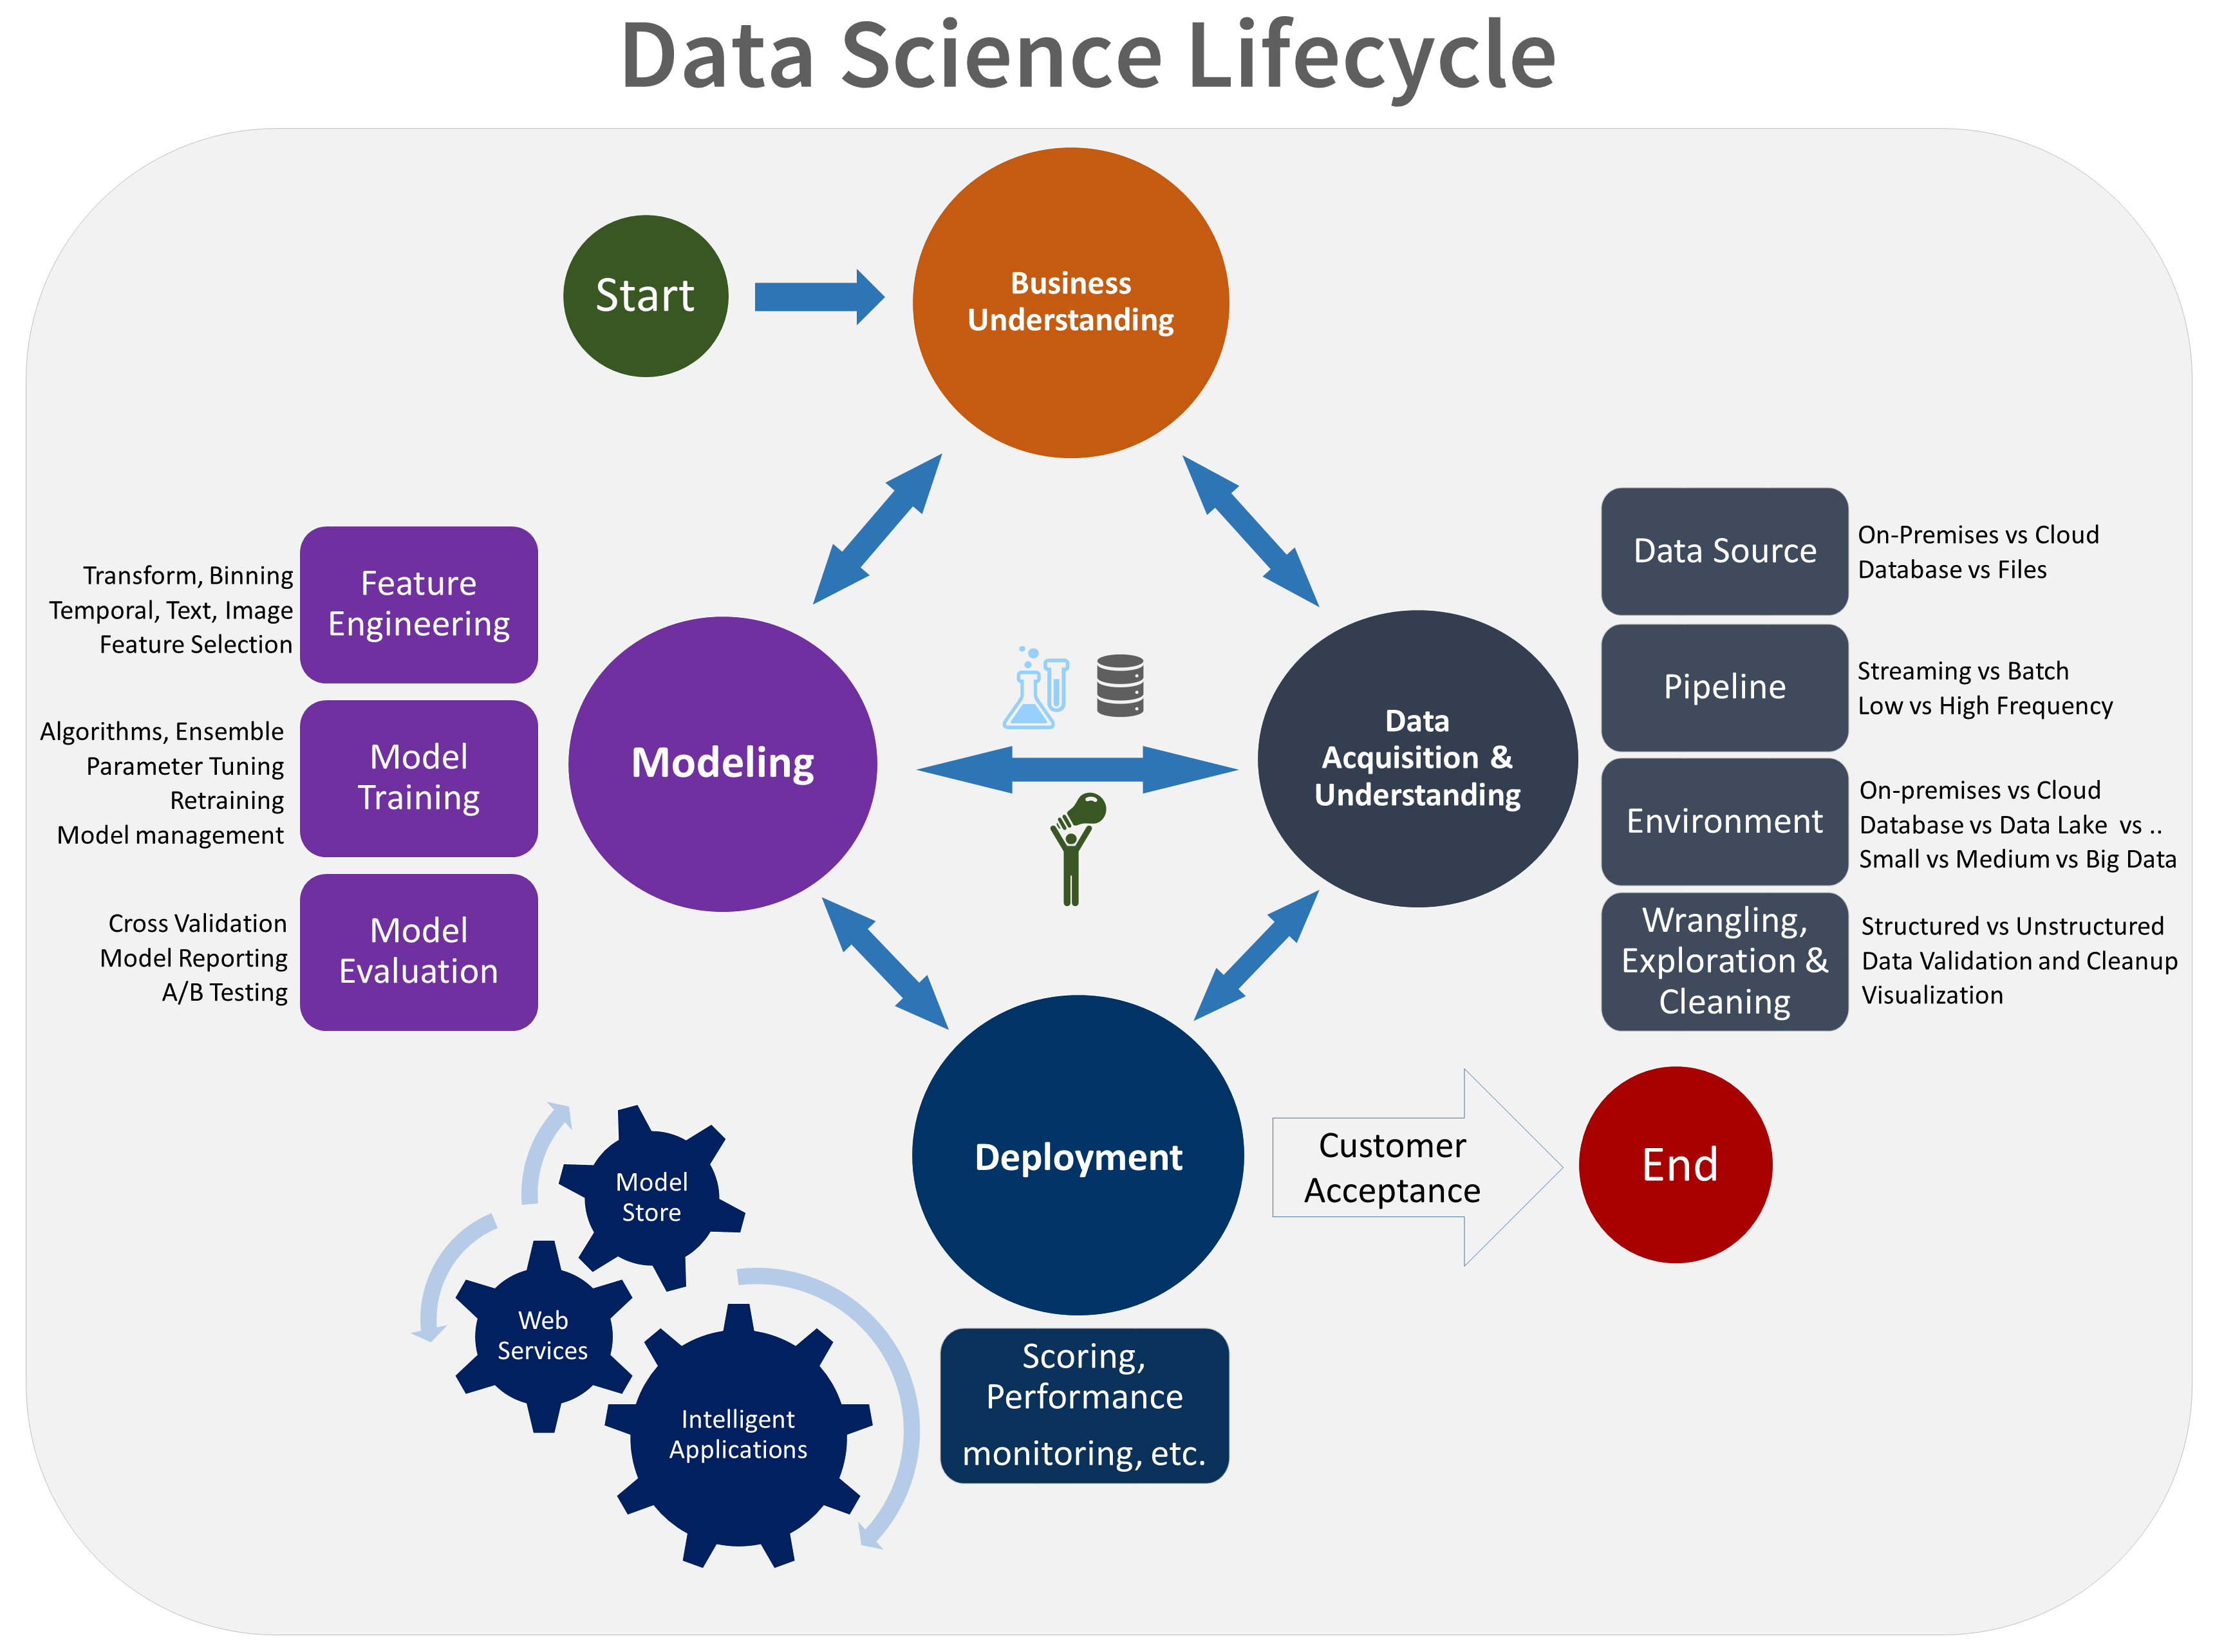
\includegraphics[width=0.9\linewidth]{../img/TDSP_Data_Science_Lifecycle.png}
    \caption{``Data life cycle'' \citep{tdsp:2024}}
    \label{fig:tdsp}
  \end{figure}

  \begin{table}[hb!]
    \setlength\extrarowheight{1em}
    \begin{center}
        \begin{tabular}{l c l}
            \hline 
            Metric & Calculations* & Description \\
            \hline
            Accuracy & $\frac{TP + TN}{TP + TN + FP + FN}$ & Fraction of predictions made correctly \\
            Precision & $\frac{TP}{TP+FP}$ & Fraction of positive predictions made correctly \\
            Recall & $\frac{TP}{TP+FN}$ & Fraction of actual positives correctly identified \\
            \hline
            \multicolumn{3}{l}{*TP=True Positives, TN=True Negatives, FP=False Positives, FN=False Negatives} \\
            \hline
        \end{tabular}
        \caption{Performance metrics used on each of the four trials.}
        \label{table:metrics}
    \end{center}
\end{table}

\clearpage



\clearpage

\section*{\center{References}}

\setcounter{page}{29}

\bibliographystyle{chicago}
\center{\bibliography{references}}



\end{document}